\documentclass[11pt, a4paper]{awesome-cv}
\fontdir[fonts/]
\newcommand*{\sectiondir}{resume/}
\colorlet{awesome}{awesome-red}
\usepackage{import}
\usepackage[none]{hyphenat}
\usepackage{graphicx}


\name{Yohann Jacob}{Sandvik}
%\address{Kvernbakken 28, 1414 Trollaasen, Norway}
\mobile{(+47) 489-58-285} 
%%% Social
\email{yohannjsandvik@gmail.com}
%\homepage{THIS_IS_A_HOMEPAGE}
% \github{yohannjs}
%\kaggle{}
\linkedin{yohann-jacob-sandvik-711073101}
%%% Optionals
% \position{Data Science{\enskip\cdotp\enskip}Computer Vision{\enskip\cdotp\enskip}Embedded Developer{\enskip\cdotp\enskip}Born June 17. 1995}



%%%%%%%%%%%%%%%%%%%%%%%%%%%%%%%%%%%%%%
%     Content
%%%%%%%%%%%%%%%%%%%%%%%%%%%%%%%%%%%%%%
%%% Make a footer for CV with three arguments(<left>, <center>, <right>)
\makecvfooter
  % {\today}
  {Yohann Jacob Sandvik}
  {\thepage}

\begin{document}
%%% Make a header for CV with personal data
%%% Add the image in the top left corner
\begin{minipage}[l]{0.2\textwidth}
  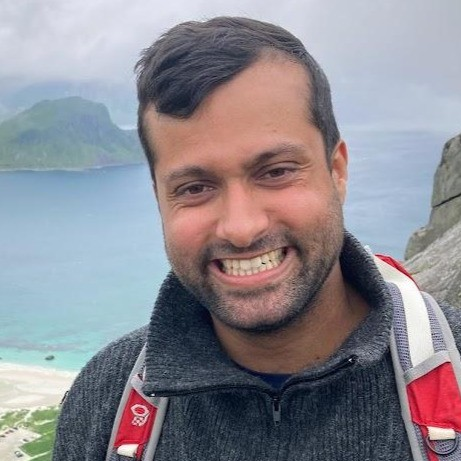
\includegraphics[width=\textwidth]{YJS.jpg} % Adjust the width as needed
\end{minipage}
\begin{minipage}[r]{0.75\textwidth}
  \makecvheader
\end{minipage}

%%% Import contents
% \import{\sectiondir}{relevant_skills.tex}
% \import{\sectiondir}{education.tex}
% \import{\sectiondir}{experience.tex}

\cvsection{Relevant skills}

\begin{cvRelevantSkills}
I have used \textbf{Python} for data science and data management. I have experience with packages in the \textbf{scipy}-stack, machine learning models in \textbf{scikit-learn} and developing deep learning models with \textbf{PyTorch} and \textbf{Tensorflow}. I am comfortable with \textbf{MATLAB}, and familiar with the \textbf{Julia} and \textbf{R} programming languages.
\newline
\newline
I have experience with the \textbf{C} programming language, and the \textbf{Git} versioning system. I am comfortable developing software in a \textbf{Linux}-based environment, and like to automate processes with \textbf{BASH} scripts. I have experience with setting up virtual software environments using \textbf{Anaconda} and \textbf{pyenv}, and configuring containers using the \textbf{Singularity} framework. I have worked in projects using the \textbf{Agile}- and \textbf{Test-driven-development} methodologies, and have used \textbf{Jira} for task management. Having both an Indian and a Norwegian parent I am also fluent in Norwegian and English. 
% \newline
% \newline
% I have designed schematics using \textbf{OrCAD Capture CIS}, and \textbf{Altium Designer}. I am fairly proficient with soldering components with a footprint as small as 0402 on PCB assemblies. I can operate equipment such as power supplies, signal generators, oscilloscopes and programmable electronic loads for testing electronics. I have done some \textbf{digital design} using \textbf{VHDL} and \textbf{SystemVerilog}.
\end{cvRelevantSkills}

\cvsection{Work experience}
\begin{cventries}
    \cventry
    {Summer Intern at System Integration Group}
    {Nordic Semiconductor ASA}
    {Kongsberg, Norway}
    {Jun. 2019 - Aug. 2019}
    {      
      \begin{cvitems}
        \item {Worked with verification of digital design.}
      \end{cvitems}
    }
    \cventry
    {Summer internship in Project Local Hawk}
    {Kongsberg Defence and Aerospace AS}
    {Kongsberg, Norway}
    {Jun. 2017 - Aug. 2017}
    {      
      \begin{cvitems}
        \item {A detailed description of the project, my tasks and my performance evaluation can be found in the work certificate from KDA.}
      \end{cvitems}
    }
    \cventry
    {Learning assistant in course tfe4172 - Introduction to Semiconductor Devices}
    {IE Faculty, NTNU}
    {Trondheim, Norway}
    {Jan. 2017 - May. 2017}
    {      
      \begin{cvitems}
        \item {The job entailed correcting student-submitted projects and supervising students with their projects.}
      \end{cvitems}
    }
    \cventry
    {Tutor in Mathematics}
    {House of Math AS}
    {Oslo, Norway}
    {Aug. 2015 - Sept. 2017}
    {
      \begin{cvitems}
        \item {I tutored in the subject of mathematics, at different levels.}
      \end{cvitems}
    }
\end{cventries}

\cvsection{Education}
\begin{cventries}
  \cventry
    {NTNU (Norwegian University of Science and Technology)}
    {MSc in Electronic Engineering}
    {Trondheim, Norway}
    {Aug. 2014 - PRESENT}
    {
      \begin{cvitems}
        \item {Title of course is ''Electronic systems design and innovation''}
        \item {With a specialization in signal processing}
        \item {With a year of exchange at EURECOM in Biot, France}
      \end{cvitems}
    }
  \cventry
    {NTNU (Norwegian University of Science and Technology)}
    {BMath in Statistics}
    {Trondheim, Norway}
    {Aug. 2017 - PRESENT}
    {
      \begin{cvitems}
        \item {Taken at the same time as the masters in electronic engineering}
      \end{cvitems}
    }
  \cventry
    {Aas Secondary High School}
    {(IBDP) International Baccalaureate Diploma Programme}
    {Aas, Norway}
    {Aug. 2011 - May. 2014}
    {
      \begin{cvitems}
        \item {With the specialization in the subjects Mathematics, Physics and Economics}
      \end{cvitems}
    }
\end{cventries}

\newpage
\cvsection{Other Experience and Skills}

\cvsubsection{Academic Work}

\begin{cvSmallExps}
    \cvSmallExp
        {2025} % Date
        {Using Deep Learning for Accurate Code-based Log Tracking from Forest to Sawmill} % Title
        {\textit{Manuscript}} % \textit{Journal}, DOI
    \cvSmallExp
        {2024} % Date
        {A Comparative Literature Review of Machine Learning and Image Processing Techniques Used for Scaling and Grading of Wood Logs} % Company
        {\textit{Forests}, 10.3390/f15071243} % Role
    \cvSmallExp
        {2020} % Date
        {Machine Learning for Classification of Myocardial Infarction and Heart failure Using Longitudinal Myocardial Strain} % Company
        {\textit{Master thesis (Grade A)}, https://hdl.handle.net/11250/2778134} % Role
\end{cvSmallExps}

\vspace{1em} % Add vertical space here

\cvsubsection{Teaching Experience}

\begin{cvSmallExps}
    \cvSmallExp
        {Lecturer} % Role
        {IMRT100 - Introductory Course, Subject-oriented Project} % Course
        {NMBU, 2023 and 2024.} % Institution and Year(s)
    \cvSmallExp
        {Lecturer} % Role
        {DAT200 - Applied Machine Learning} % Course
        {NMBU, 2024} % Institution, Year(s)
    \cvSmallExp
        {Teaching assistant} % Role
        {DAT300 - Applied Deep Learning} % Course
        {NMBU, 2022, 2023 and 2024} % Institution, Year(s)
    \cvSmallExp
        {Teaching assistant} % Role
        {TFE4172 - Introduction to Semiconductor Devices} % Course
        {NTNU, 2020} % Institution, Year(s)
    \cvSmallExp
        {Teaching assistant} % Role
        {TFE4280- Sensors and Instrumentation} % Course
        {NTNU, 2017} % Institution, Year(s)
\end{cvSmallExps}

\vspace{1em} % Add vertical space here

\cvsubsection{Languages}

\begin{cvSmallExps}
    \cvSmallExp
        {Fluent in}
        {Norwegian and English}
        {} 
    \cvSmallExp
        {Familiar with}
        {German and French}
        {}
\end{cvSmallExps}

\vspace{1em} % Add vertical space here

\cvsubsection{Volunteer Roles}

\begin{cvSmallExps}
    \cvSmallExp
        {2017} % Date
        {E\&T dagene} % Company
        {Head of the Business Contacts group at the student career fair.} % Role
    \cvSmallExp
        {2016} % Date
        {NTNUI Jiu Jitsu} % Company
        {Was responsible for managing the clubs finances for a year.} % Role
    \cvSmallExp
        {2014 - 2015} % Date
        {Omega (student union)} % Company
        {Part of the founding members of the student union's brewing committee} % Role
\end{cvSmallExps}


\end{document}
